\chapter{Introduction}

\vspace{0.5cm}

As we enter the more "technical" aspect of this thesis, a brief introduction is necessary. This part of the thesis
(and Part \ref{part:visitor-and-visualising}) will present several Python "modules". Each one of them builds upon the previous one to
add more functionality, but all are layers can be run as-is, not only the last one.\newline

The following diagram explains how these modules interact with each other:\newline

\begin{figure}[H]
%\centering
\hspace{-1.5cm}
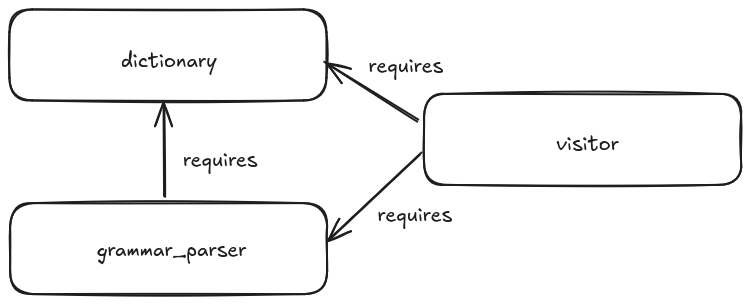
\includegraphics[scale=0.43]{images/module_dependency.png}
\caption{Dependency between the created Python modules}
\end{figure}

The modules are the following: \newline

\begin{itemize}
\item The \textbf{"dictionary"} module: Described in Chapter \ref{chap:creating_a_dictionary},
this module allows to get definitions for Lojban words, as well as some structural elements;
\item The \textbf{"grammar\_parser"} module: Described in Chapter \ref{chap:parser}, this module parses
a Lojban sentence to check its validity, and returns its Parsing Tree;
\item The \textbf{"visitor"} module: Described in Chapter \ref{chap:visitor-module}, this module goes through
a sentence's Parsing Tree and highlights nodes of relevance, in order to tag parts of speech or assign a semantic role
to words in a sentence;
\item The \textbf{"visualize"} module: Described in Chapter \ref{chap:visualize-module}, this module takes the
representation of the sentence created by the previous module and displays it in a more visual and interactive way.
\end{itemize}

Additionally a \textbf{"tests"} folder, described in Chapter \ref{chap:creating_a_test_suite}, contains code to
test the validity of the Parsing Expression Grammar created in Part \ref{part:creating-a-peg} of the thesis, by
running the grammar\_parser module several times against a big collection of Lojban sentences.\newline

Our main companion through the development of these tools is the Parsimonious Python library \footcite{parsimonious}.
Although its maintenance is rather sporadic (only one commit so far in 2024, at the time of writing), it was picked because of
several selling points:

\begin{itemize}
\item it is fast;
\item has an dense set of features (which will be presented in later chapters);
\item good error reporting
\end{itemize}

One of its main flaws, however, is the lack of proper documentation. A lot of the code is self-documented, but intense
trial and error is required to understand fully how the library's API can be used effectively. But once understood, the
benefits outweigh the costs, and that is why this library was selected instead of other more famous ones in the Python ecosystem.